\chapter{Analisis}
Pada bab ini penulis akan membahas analisis masalah yang mungkin ada pada algoritma. Masalah yang mungkin akan dihadapi adalah beberapa kata yang ada pada \textit{stego cover} memiliki sinonim dengan banyak suku kata yang sama dengan kata aslinya(yang ada pada \textit{stego cover}). Selain itu juga \textit{stego cover} dapat berisi nama orang, sehingga tidak memiliki sinonim.

\section{Hipotesis}

\subsection{Pemenggalan Kata}
Untuk proses pemenggalan kata, akan menggunakan skripsi Frisca Sumarlin 2010 yang berjudul Aplikasi Pendongeng. Untuk mengenali suku kata dalam bahasa Indonesia, akan digunakan tiga tahap DFSA. Setiap masukan dari DFSA merupakan hasil DFSA tahap sebelumnya. Seperti yang telah dijelaskan , FSA memiliki prinsip kerja membaca hanya satu arah dan tidak bisa membaca mundur masukannya. Sedangkan untuk mengenali suku kata, untuk beberapa kasus kata dibutuhkan kemampuan untuk membaca mundur masukannya. Sebagai contoh, pada kata "anda", huruf ketiga adalah huruf konsonan sehingga pemenggalan suku kata dapat dilakukan pada saat membaca huruf ketiga. Berbeda dengan kata "anda", pada kata "alis", huruf ketiga adalah huruf vokal, \textit{automaton} harus mundur untuk melakukan pemenggalan suku kata.

Pada tahap 1 ini memang belum sesuai dengan aturan penyukuan kata yang benar, karena itu akan dilakukan tiga tahapan. Untuk diagramnya dapat dilihat pada gambar \ref{fig:1-DFSA-1}.

\begin{figure}[H]
	\centering
	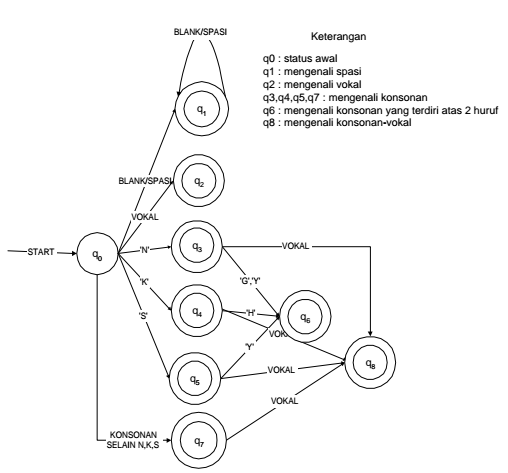
\includegraphics[scale=1.3]{Gambar/DFSA-1}
	\caption{Diagram Transisi DFSA tahap 1\cite{Thomas:2000}} 
	\label{fig:1-DFSA-1}
\end{figure}

Penjelasan tentang \ref{fig:1-DFSA-1}Diagram Transisi DFSA tahap 1 untuk mengenali spasi, vokal(V), konsonan yang terdiri dari 1 huruf (K), konsonan yang terdiri dari 2 huruf (KK), dan konsonan-vokal (KV) adalah sebagai berikut.

\begin{itemize}
	\item Perpindahan dari status awal (\textit{q0}) ke \textit{q1} adalah untuk mengenali spasi atau \textit{string} kosong.
	\item Perpindahan dari \textit{q0} ke \textit{q2} adalah untuk mengenali huruf vokal.
	\item Perpindahan dari \textit{q0} ke \textit{q3} adalah untuk mengenali huruf 'N'.
	\item Perpindahan dari \textit{q0} ke \textit{q4} adalah untuk mengenali huruf 'K'.
	\item Perpindahan dari \textit{q0} ke \textit{q5} adalah untuk mengenali huruf 'S'.
	\item Perpindahan dari \textit{q0} ke \textit{q7} adalah untuk mengenali huruf konsonan selain 'N', 'K', dan 'S'.
	\item Perpindahan dari \textit{q3} ke \textit{q8} adalah untuk mengenali pola suku kata VK.
	\item Perpindahan dari \textit{q3} ke \textit{q6} adalah untuk mengenali pola suku kata KK (ng dan ny).
	\item Perpindahan dari \textit{q3} ke \textit{q8} adalah untuk mengenali pola suku kata KV.
	\item Perpindahan dari \textit{q4} ke \textit{q6} adalah untuk mengenali pola suku kata KK (kh).
	\item Perpindahan dari \textit{q4} ke \textit{q8} adalah untuk mengenali pola suku kata KV.
	\item Perpindahan dari \textit{q5} ke \textit{q6} adalah untuk mengenali pola suku kata KK (sy).
	\item Perpindahan dari \textit{q5} ke \textit{q8} adalah untuk mengenali pola suku kata KV.
	\item Perpindahan dari \textit{q7} ke \textit{q8} adalah untuk mengenali pola suku kata KV.
\end{itemize}

Sebagai contoh, jika melakukan pemenggalan kata hanya dengan menggunakan \ref{fig:1-DFSA-1}DFSA tahap 1 saja, kata "gondok" tidak dapat dipotong secara sempurna. Berikut langkah-langkahnya.

\begin{itemize}
	\item Pada status awal (\textit{q0}) huruf ke-1 'g' akan diperiksa.
	\item Pindah ke \textit{q7} karena huruf 'g' merupakan huruf konsonan selain huruf 'N', 'K', dan 'S'.
	\item Huruf ke-2 'o' diperiksa dan pindah ke \textit{q8} karena huruf 'o' merupakan huruf vokal. Suku kata ke-1 "go" disimpan, lanjut ke huruf selanjutnya dan mulai lagi dari \textit{q0}.
	\item Huruf ke-3 'n' diperiksa dan pindah ke \textit{q3} karena huruf ke-3 adalah huruf 'n'.
	\item Huruf ke-4 'd' diperiksa dan tidak memenuhi syarat untuk ke \textit{q8} ataupun \textit{q6}. Suku kata ke-2 "n" disimpan. Huruf ke-4 'd' kembali ke \textit{q0}.
	\item Pindah ke \textit{q7} karena huruf 'd' merupakan huruf konsonan selain huruf 'N', 'K', dan 'S'.
	\item Huruf ke-5 'o' diperiksa dan pindah ke \textit{q8} karena '0' merupakan huruf vokal. Suku kata ke-3 "do" disimpan, lanjut ke huruf selanjutnya dan mulai lagi dari \textit{q0}.
	\item Huruf ke-6 'k' diperiksa dan pindah ke \textit{q4} karena huruf ke-6 adalah huruf 'K'. Suku kata ke-4 "k" disimpan. Tahap 1 selesai karena semua huruf telah melewati diagram transisi DFSA tahap 1.
	\item Didapatkan hasil pemenggalan suku kata "gondok" menjadi "go-n-do-k".
\end{itemize}

Dapat dilihat bahwa jika hanya menggunakan \ref{fig:1-DFSA-1}DFSA tahap 1, hasilnya masih belum sempurna. Pada tahan 1 hanya dikenali pola suku kata V, K, KV, dan KK. Selanjutnya, setelah melewati tahapan 1 DFSA, \textit{output}nya akan menjadi masukan untuk DFSA tahap 2. Pada tahap 2 ini harus dikenali V, KV, dan pengembangan dari ketiga pola yang dikenali pada tahap pertama. Pada tahap ini, pengembangan yang bisa dilakukan adalah V+K, K+KV, K+KV+K, K+K+KV, K+K+KV+K, K+KV+K, dan KV+K. Untuk digram transisi tahap kedua dapat dilihat pada gambar \ref{fig:2-DFSA-2}.

\begin{figure}[H]
	\centering
	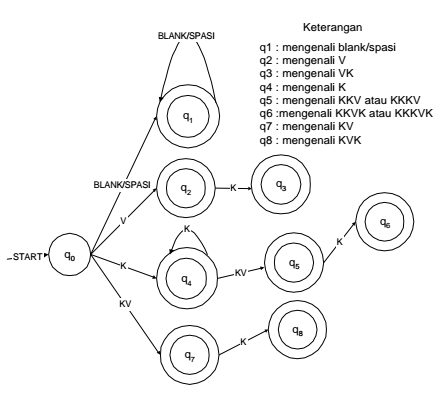
\includegraphics[scale=1.3]{Gambar/DFSA-2}
	\caption{Diagram Transisi DFSA tahap 2\cite{Thomas:2000} 
	\label{fig:2-DFSA-2}}
\end{figure}

Penjelasan tentang \ref{fig:1-DFSA-2}Diagram Transisi DFSA tahap 2 untuk mengenali pola suku kata V, VK, K, KKV, KKKV, KKVK, KKKVK, KV, dan KVK adalah sebagai berikut.

\begin{itemize}
	\item Perpindahan dari status awal (\textit{q0}) ke \textit{q1} adalah untuk mengenali spasi atau \textit{string} kosong.
	\item Perpindahan dari \textit{q0} ke \textit{q2} adalah untuk mengenali pola suku kata V.
	\item Perpindahan dari \textit{q0} ke \textit{q4} adalah untuk mengenali pola suku kata K.
	\item Perpindahan dari \textit{q0} ke \textit{q7} adalah untuk mengenali pola suku kata KV.
	\item Perpindahan dari \textit{q2} ke \textit{q3} adalah untuk mengenali pola suku kata VK.
	\item Perpindahan dari \textit{q4} ke \textit{q4} adalah untuk mengenali pola suku kata KK.
	\item Perpindahan dari \textit{q4} ke \textit{q5} adalah untuk mengenali pola suku kata KKV atau KKKV.
	\item Perpindahan dari \textit{q5} ke \textit{q6} adalah untuk mengenali pola suku kata KKVK atau KKKVK.
	\item Perpindahan dari \textit{q7} ke \textit{q8} adalah untuk mengenali pola suku kata KVK.
\end{itemize}

Pada tahap 2, masih ada tiga pola suku kata yang belum dapat dikenali, yaitu VKK, KVKK, dan KKVKK. Untuk itu masih dibutuhkan satu tahapan lagi untuk dapat mengenali pola-pola tersebut dan mengenali huruf diftong. Pada tahap ini hasil dari DFSA tahap kedua akan menjadi masukan bagi DFSA tahap terakhir yaitu tahap 3.

\begin{figure}[H]
	\centering
	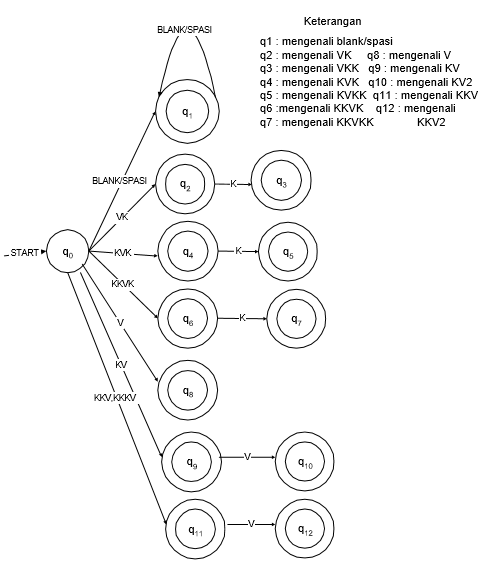
\includegraphics[scale=1.3]{Gambar/DFSA-3}
	\caption{Diagram Transisi DFSA tahap 3\cite{Thomas:2000}} 
	\label{fig:3-DFSA-3}
\end{figure}

Penjelasan tentang \ref{fig:1-DFSA-3}Diagram Transisi DFSA tahap 3 untuk mengenali pola suku kata VK, V, VKK, KV, KVK, KVV, KVKK, KKV, KKVK, KKVKK, dan KKVV adalah sebagai berikut.

\begin{itemize}
	\item Perpindahan dari status awal (\textit{q0}) ke \textit{q1} adalah untuk mengenali spasi atau \textit{string} kosong.
	\item Perpindahan dari \textit{q0} ke \textit{q2} adalah untuk mengenali pola suku kata VK.
	\item Perpindahan dari \textit{q0} ke \textit{q4} adalah untuk mengenali pola suku kata KVK.
	\item Perpindahan dari \textit{q0} ke \textit{q6} adalah untuk mengenali pola suku kata KKVK.
	\item Perpindahan dari \textit{q0} ke \textit{q8} adalah untuk mengenali pola suku kata V.
	\item Perpindahan dari \textit{q0} ke \textit{q9} adalah untuk mengenali pola suku kata KV.
	\item Perpindahan dari \textit{q0} ke \textit{q11} adalah untuk mengenali pola suku kata KKV atau KKKV.
	\item Perpindahan dari \textit{q2} ke \textit{q3} adalah untuk mengenali pola suku kata VKK.
	\item Perpindahan dari \textit{q4} ke \textit{q5} adalah untuk mengenali pola suku kata KVKK.
	\item Perpindahan dari \textit{q6} ke \textit{q7} adalah untuk mengenali pola suku kata KKVKK.
	\item Perpindahan dari \textit{q9} ke \textit{q10} adalah untuk mengenali pola suku kata KVV.
	\item Perpindahan dari \textit{q11} ke \textit{q12} adalah untuk mengenali pola suku kata KKVV atau KKKVV.
\end{itemize}

Untuk dapat membagi suku kata, diperlukan automata yang dapat menerima masukan berupa kata dan keluaran berupa suku kata. \textit{Finite State Transducer} merupakan \textit{finite state machine} yang memiliki dua pita, yaitu pita masukan dan pita keluaran. Automata yang telah dirancang adalah DFSA, di mana keluaran yang dihasilkan adalah dikenali atau tidak dikenali. Dengan merubah keluaran dari DFSA tersebut menjadi suku kata untuk setiap sekuens karakter yang telah dikenali, maka DFSA yang telah dirancang dapat dimanfaatkan untuk membagi kata menjadi suku kata. Atas dasar itu, DFSA dipilih untuk melakukan penyukuan kata.

Pemenggalan suku kata akan dipakai untuk mendapatkan banyak suku kata kata-kata yang terdapat pada \textit{stego cover}, sehingga dapat dihitung banyak suku kata tiap katanya. Namun karena kumpulan \textit{stego cover} yang akan dipakai dapat berupa cerita pendek(cerpen) atau puisi, maka isi dari \textit{stego cover} tidak hanya berupa kata-kata alfabet saja, tetapi juga ada angka yang bisa berupa tanggal, kata serapan, dan lain-lain. Hal ini kemudian dapat menjadi hambatan, karena seperti yang kita ketahui bahwa angka tidak memiliki suku kata. Hambatan lainnya juga datang dari kata-kata dalam bahasa asing dan singkatan.

Setelah menemui hambatan-hambatan di atas, akhirnya diputuskan beberapa solusi. Pertama-tama, dari keseluruhan isi \textit{stego cover}, tanda baca akan diabaikan(kecuali tanda penghubung '-'), sehingga yang akan dipenggal hanyalah kata-katanya saja. Semua angka akan dianggap sebagai satu suku kata. Semua singkatan atau kata dalam bahasa asing, akan dilakukan pemenggalan kata apa adanya.

\subsection{\textit{Database} kata}
Penyisipan akan memanfaatkan pasangan kata yang memiliki suku kata berbeda, namun memiliki arti yang sama atau serupa. \textit{Database} kata akan disimpan dalam sebuah \textit{file} dengan ekstensi .txt. Pada \textit{file} tersebut satu per satu kata yang ada pada \textit{stego cover} memiliki sinonimnya sendiri. Pencarian sinonim pertama-tama akan dicari pada Tesaurus. Tesaurus \footnote{http://kbbi.web.id/tesaurus}merupakan buku referensi berupa daftar kata dengan sinonimnya. Kata-kata yang terdaftar di Tesaurus adalah kata baku, sehingga jika pada \textit{stego cover} terdapat kata yang tidak dapat ditemukan pada Tesaurus, diperlukan penanganan tersendiri.

Solusinya adalah dengan mengubah-ubah imbuhan pada awal atau akhir kalimat, namun tetap memperhatikan konteks kalimat tersebut. Sebagai contoh, pada \textit{stego cover} terdapat kata 'menggendongnya', namun kata tersebut tidak dapat ditemukan pada Tesaurus, karena terdapat imbuhan. Sehingga untuk sinonimnya dapat digunakan kata 'menggendong'. Kedua kata tersebut memiliki jumlah suku kata yang berbeda, namun memiliki arti yang sama.

Terdapat beberapa kata yang memang tidak memiliki sinonim dengan jumlah suku kata yang berbeda. Kata 'lama' memiliki 2 suku kata, sedangkan sinonim yang ada pada Tesaurus adalah 'lamban' dan 'lelet'. Kedua sinonimnya memiliki suku kata yang genap, tetapi yang dibutuhkan adalah yang bersuku kata ganjil. Hal ini dapat diatasi dengan menyamarkannya sebagai \textit{typo} atau kesalahan pengetikkan. Contohnya dengan memasukkan kata 'lambaan' atau 'lamaa' sebagai sinonim dari kata 'lama'. Kata 'lambaan' dan 'lamaa', jika dipotong suku katanya dengan menggunakan pemotong suku kata yang telah dibuat, kedua kata tersebut memiliki suku kata ganjil.

\subsection{Stego Cover}
\textit{Stego cover} yang telah dikumpulkan berupa puisi dan cerpen. Alasan dipilihnya cerpen dan puisi sebagai \textit{stego cover}, karena puisi umumnya menggunakan satu kata berulang-ulang, sehingga dapat mengurangi banyaknya kata yang disimpan pada \textit{file database}. Sedangkan cerpen yang dipilih memiliki jumlah kata yang cukup banyak, ini menandakan kapasitas penyimpanan yang cukup besar.

Dengan dipilihnya cerpen dan puisi sebagai \textit{stego cover}, maka dibutuhkan skema komunikasi yang dapat menyamarkan artikel tersebut agar tidak menimbulkan kecurigaan oleh pihak lain. Skema komunikasi yang dipilih berupa komunikasi antara dua mahasiswa yang gemar mengirim puisi atau cerpen melalui \textit{email}. \textit{Email} yang dikirim mengandung \textit{stego object} yang merupakan hasil dari penyisipan \textit{secret message} pada \textit{stego cover}. Dengan skema komunikasi seperti ini, jika ada pihak lain yang membaca \textit{email} kedua mahasiswa tersebut, tidak akan mencurigai adanya kejanggalan karena kedua mahasiswa gemar berkirim puisi dan cerpen.

\subsection{Penyisipan}
Proses steganografi akan memanfaatkan suku kata dan sinonim kata itu sendiri. Ide utamanya adalah dengan mengganti kata-kata tertentu yang ada dalam \textit{stego cover} dengan kata-kata yang telah disediakan pada \textit{file database}. File \textit{database} berisi semua kata yang ada pada \textit{stego cover} berpasangan dengan sinonimnya. Pasangan kata yang ada pada \textit{database} merupakan sinonim dengan banyak suku kata yang berbeda(ganjil dan genap) dengan kata aslinya.

Penggantian kata pada \textit{stego cover} ditentukan dari ASCII \textit{secret message} yang akan disisipkan. ASCII\footnote{http://whatis.techtarget.com/definition/ASCII-American-Standard-Code-for-Information-Interchange} (\textit{American Standard Code for Information Interchange}) merupakan format yang paling umum untuk file teks yang ada di komputer dan internet. Kode ASCII yang akan dipakai direpresentasikan dengan 7-bit angka biner, yang berarti ada 7 digit angka 0 atau 1. Pemilihan 7-bit ini dikarenakan kode ASCII pada bilangan desimal hanya ada dari 0 sampai 127, sehingga jika menggunakan 8-bit, angka pertama(paling kiri) akan selalu bernilai 0. Dapat disimpulkan bahwa untuk menyisipkan 7-bit dibutuhkan 7 kata, 8-bit dibutuhkan 8 kata.  Untuk alasan memaksimalkan kapasitas penyisipan, maka diputuskan untuk merepresentasikan 1 karakter menjadi 7-bit.

Setelah \textit{secret message} diubah menjadi deretan kode ASCII, satu per satu digit kodenya akan dicocokkan dengan banyaknya suku kata pada \textit{stego cover}. Kode digit pertama akan disisipkan pada kata pertama \textit{stego cover}, digit kedua disisipkan pada kata kedua, dst. Jika banyak suku kata pada \textit{stego cover} tidak sesuai dengan kode, maka kata tersebut akan dicari sinonimnya pada \textit{file database}, jika ditemukan kata dengan banyak suku kata yang sesuai dengan kode, maka kata tersebut akan diganti. Pemberitahuan akan muncul jika kata yang tidak sesuai kode tidak memiliki sinonim pada \textit{file database}.

\subsubsection{Algoritma}
Seperti yang telah dijelaskan sebelumnya, algoritma ini akan memanfaatkan kata yang ada pada \textit{stego cover} untuk menyisipkan kode ASCII dari pesan rahasia. Proses penyisipan ini juga memanfaatkan \textit{file database} untuk mengubah kata asli yang ada pada \textit{stego cover} dengan kata sinonim yang ada pada \textit{file database} jika banyak suku kata tidak sesuai dengan kode ASCII pesan rahasia.

Algoritma penyisipan pesan rahasia pada \textit{stego cover} dengan memanfaatkan sinonim

\begin{enumerate}
	\item Meminta input berupa pesan rahasia(\textit{secret}).
	\item Tiap karakter pada \textit{secret} diubah menjadi kode ASCII 7-bit dan disimpan menjadi \textit{secret code}.
	\item Hitung berapa banyak angka yang ada pada \textit{secret code}.
	\item Cari \textit{stego cover} yang dapat menampung \textit{secret code}.(Banyaknya kata yang ada dalam \textit{stego cover} > banyak angka yang ada pada \textit{secret code}).
	\item Bangkitkan angka acak dari 0 sampai banyaknya \textit{stego cover} yang dapat menampung \textit{secret code}. Angka acak ini dinamakan \textit{random}.
	\item Buka file ke-\textit{random} dan baca per kata dengan mengabaikan tanda baca dan spasi.
	\item Untuk tiap kata ke-n, lakukan pemenggalan kata dan hitung banyaknya suku kata pada kata ke-n tersebut dan lakukan operasi \textit{mod} 2. Hasil operasi ini dinamakan banyakSK.
	\item Cocokkan banyakSK dengan angka ke-n yang ada pada \textit{secret code} secara berurutan.(banyakSK kata ke-n dicocokkan dengan angka ke-n \textit{secret code})
	\item Jika pada tahap 7 didapatkan banyakSK yang tidak sesuai dengan angka ke-n \textit{secret code}, lanjut ke tahap 9. Jika sesuai, ulangi tahap 7 sampai semua angka pada \textit{secret code} berhasil disisipkan.
	\item Cari sinonim kata tersebut pada \textit{file database}. Kata yang diambil hanya kata dengan banyakSK yang memiliki nilai berbeda.
	\item Dari kata-kata yang didapatkan dari tahap 10, akan dilakukan pengambilan kata secara acak.
	\item Kata yang telah diambil dari tahap 11, akan menggantikan kata yang tidak sesuai sebelumnya.
\end{enumerate}

\subsection{Ekstraksi Pesan Rahasia}
Pada proses pengekstraksian kembali pesan rahasia akan dibutuhkan input berupa \textit{stego-object} yang merupakan hasil dari penyisipan. Perangkat pertama-tama akan membaca secara keseluruhan inputnya, lalu melakukan pemenggalan kata sama seperti yang dilakukan pada saat proses penyisipan. Selesai melakukan pemenggalan kata, banyak suku kata tiap katanya akan dihitung dan dilakukan operasi \textit{mod} 2 sehingga didapatkan angka 0 dan 1. Saat ini telah didapatkan deretan angka 0 dan 1 yang dinamakan \textit{secret code}. Saat menyisipkan memang 1 karakter diubah menjadi kode ASCII 7-bit, namun \textit{java} menyediakan fungsi untuk mengubah deret biner 8-bit menjadi karakter. Sehingga untuk setiap 7-bit pada \textit{secret code} dapat ditambahkan angka 0 di paling kiri sebelum dijadikan \textit{input} pada fungsi \textit{java} tersebut.

Setelah selesai mengubah bit-bit yang ada menjadi karakter, hasilnya akan ditampilkan pada layar. Proses ektraksi ini melibatkan semua kata yang ada pada \textit{stego-object}, sehingga kata yang tidak disisipkan pesan rahasia pun ikut terekstraksi. Hasilnya pesan rahasia yang diekstrak, dapat menampilkan karakter-karakter yang tidak memiliki arti. Hal ini dibiarkan agar penerima \textit{stego-object} dapat mengekstraksi pesan rahasia tanpa memerlukan informasi apapun. Alasan lainnya juga agar \textit{stego cover} dapat memaksimalkan kapasitas penyisipan.

\section{Analisis Use Case}

Diagram \textit{use case} perangkat lunak steganografi ini memiliki satu aktor, yaitu pengguna. Berikut diagram \textit{usecase} dari perangkat lunak yang akan dibangun.

\begin{figure}[H]
	\centering
	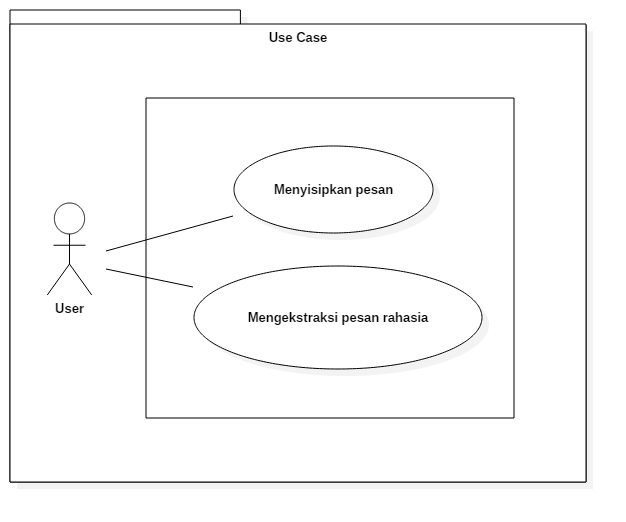
\includegraphics[scale=0.5]{Gambar/usecase}
	\caption{Use Case Diagram Perangkat Lunak Steganografi} 
	\label{fig:3_usecase}
\end{figure}

Dari diagram di atas dapat dilihat dua \textit{use case}, yakni:
\begin{enumerate}
	\item \textbf{Menyisipkan pesan}, pengguna mengetikkan pesan rahasia yang akan disisipkan.
	\item \textbf{Mengekstraksi kembali pesan rahasia}, pengguna akan memasukkan \textit{stego-object} yang diterima.
\end{enumerate}

\subsection{Skenario Use Case}

\begin{enumerate}
	\item \textbf{Menyisipkan pesan}
	\begin{itemize}
		\item Nama: Menyisipkan pesan
		\item Aktor: Pengguna
		\item Deskripsi: Mengetikkan pesan rahasia yang akan disisipkan		
		\item Prakondisi: -
		\item Tujuan: Menyisipkan pesan rahasia yang diketikkan ke dalam salah satu dokumen yang ada di dalam dokumen korpus
		\item Skenario:
			\begin{enumerate}
				\item Pengguna mengetikkan pesan rahasia yang akan disisipkan
				\item Pengguna menekan tombol sisipkan
				\item Sistem lalu akan mengubah pesan yang diketik menjadi kode ASCII
				\item Sistem mencari dokumen yang cocok dengan kode ASCII pesan rahasia
				\item \textit{Stego-object} sebagai hasil dari penyisipan akan muncul pada layar.
			\end{enumerate}
	\end{itemize}
	
	\item \textbf{Mengekstraksi pesan rahasia}
	\begin{itemize}
		\item Nama: Mengekstraksi pesan rahasia
		\item Aktor: Pengguna
		\item Deskripsi: Memasukkan \textit{stego-object} yang didapatkan
		\item Prakondisi: Telah memiliki \textit{stego-object} yang dihasilkan dari perangkat lunak ini
		\item Tujuan: Mengkestraksi pesan rahasia yang telah disisipkan sebelumnya
		\item Skenario:
			\begin{enumerate}
				\item Pengguna menyalin \textit{stego-object} yang didapat dari perangkat yang sama
				\item Pengguna menekan tombol Ekstrak
				\item Sistem akan melakukan penyukuan kata
				\item Masing-masing kata akan dijumlahkan suku katanya
				\item Sistem menyandikan jumlah suku kata yang genap menjadi 0 dan yang ganjil menjadi 1
				\item Sistem akan mengubah deret biner menjadi karakter yang sesuai dengan kode ASCII
				\item Pesan rahasia akan ditampilkan pada layar
			\end{enumerate}
	\end{itemize}
\end{enumerate}

\subsection{Analisis Diagram Kelas}

Diagram kelas perangkat lunak steganografi dapat dilihat pada \ref{fig:3_classdiagram}

\begin{figure}[H]
	\centering
	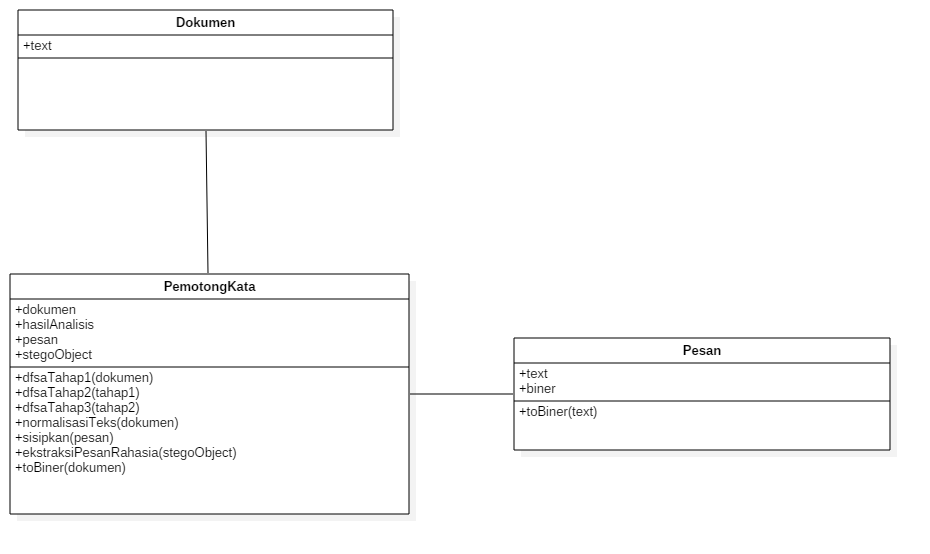
\includegraphics[scale=0.5]{Gambar/classdiagram}
	\caption{Class Diagram perangkat lunak steganografi} 
	\label{fig:3_classdiagram}
\end{figure}

Keterangan atas diagram kelas akan dijelaskan sebagai berikut:

\begin{enumerate}
	\item \textbf{Kelas Dokumen}
	\begin{itemize}
		\item Atribut text, untuk menampung teks dari dokumen berupa string
	\end{itemize}
	\item \textbf{Kelas Pesan}
	\begin{itemize}
		\item Atribut text, untuk menampung teks dari pesan berupa string
		\item Atribut biner, untuk menampung teks dari pesan berupa biner, tetapi dalam bentuk string
		\item Fungsi toBiner, memiliki parameter text. Fungsi ini akan merubah tiap karakter yang ditampung di atribut text menjadi kode ASCII dalam bentuk biner.
	\end{itemize}
	\item \textbf{Kelas PemotongKata}
	\begin{itemize}
		\item Atribut dokumen, untuk menampung isi dokumen
		\item Atribut hasilAnalisis, untuk menyimpan hasil dari penyukuan kata
		\item Atribut pesan, untuk menyimpan pesan rahasia yang akan disisipkan
		\item Atribut stegoObject, untuk menyimpan stego-object yang akan diektraksi
		\item Fungsi dfsaTahap1, memiliki parameter dokumen menghasilkan keluaran berupa hasil proses dfsa tahap pertama
		\item Fungsi dfsaTahap2, memiliki parameter tahap1 yang merupakan keluaran dfsaTahap1 dan mengeluarkan hasil proses dfsa tahap kedua
		\item Fungsi dfsaTahap3, memiliki parameter tahap2 yang merupakan keluaran dfsaTahap2 dan mengeluarkan hasil penyukuan kata dari text
		\item Fungsi normalisasiText, memiliki parameter dokumen dan menghasilkan keluaran berupa teks tanpa tanda baca dan simbol, sehingga siap untuk dipotong berdasarkan suku katanya
		\item Fungsi sisipkan, memiliki parameter pesan yang merupakan pesan rahasia yang diketikkan oleh pengguna dan akan mengeksekusi rangkaian penyisipan pesan
		\item Fungsi ekstraksiPesanRahasia, memiliki parameter stegoObject yang merupakan \textit{stego-object} yang disalin oleh pengguna dari hasil penyisipan menggunakan perangkat lunak yang sama dan akan mengeksekusi rangkaian pengekstraksian kembali pesan rahasia
		\item Fungsi toBiner, memiliki parameter dokumen. Parameter dokumen merupakan dokumen yang telah dilakukan penyukuan, sehingga fungsi ini hanya menghitung jumlah suku kata untuk setiap katanya. Jumlah kata akan disandikan dengan 0 untuk jumlah genap dan 1 untuk jumlah ganjil
	\end{itemize}
	
\end{enumerate}

\subsection{Analisis Diagram Aktivitas}

Diagram aktivitas dari perangkat lunak dibagi menjadi dua. Diagram aktivitas saat menyisipkan pesan dapat dilihat pada \ref{fig:4_activity-penyisipan}

\begin{figure}[H]
	\centering
	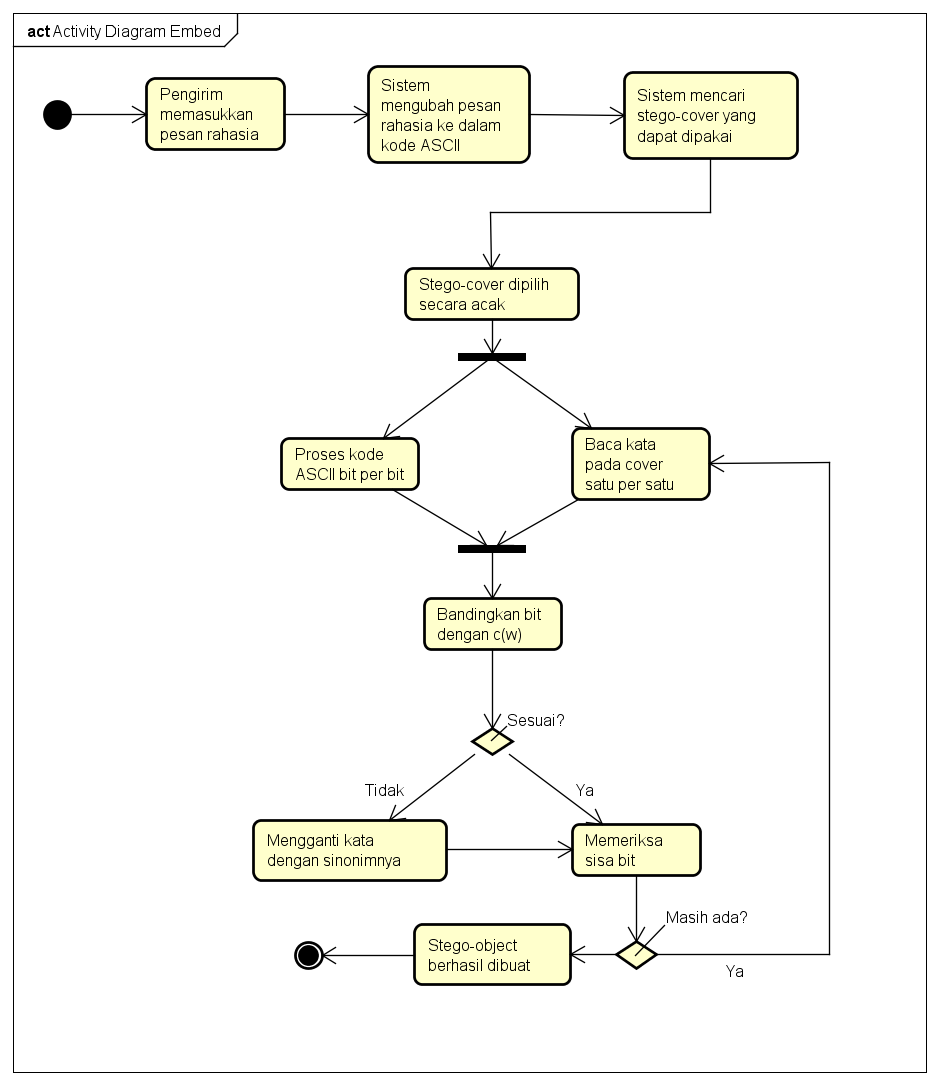
\includegraphics[scale=0.5]{Gambar/activity-penyisipan}
	\caption{Activity Diagram perangkat lunak steganografi saat menyisipkan} 
	\label{fig:4_activity-penyisipan}
\end{figure}

Dari diagram aktivitas dapat dijelaskan sebagai berikut:

\begin{enumerate}
	\item Pengguna memasukkan input berupa string (pesan rahasia)
	\item Pesan akan diubah ke bentuk ASCII
	\item Dokumen korpus akan dibuka satu per satu
	\item Untuk setiap dokumen yang dibuka akan dilakukan penyukuan kata dan dilakukan penyandian. Angka 1 untuk kata dengan jumlah suku kata genap dan angka 2 untuk kata dengan jumlah suku kata ganjil
	\item Pesan rahasia yang telah diubah ke bentuk ASCII dan dokumen yang telah disandikan akan dibandingkan. Dari sini akan dihasilkan dua kemungkinan:
	\begin{itemize}
		\item Jika ditemukan dokumen cocok dengan pesan rahasia, akan diambil kalimat yang sesuai
		\item Jika tidak ditemukan dokumen yang cocok, dari dokumen yang paling mirip akan dilakukan modifikasi (perubahan sinonim atau perubahan kalimat aktif/pasif)
	\end{itemize}
	\item Jika telah didapatkan kalimat yang sesuai, kalimat akan ditampilkan dan program selesai
\end{enumerate}

Diagram aktivitas ekstraksi dapat dilihat pada 

\begin{figure}[H]
	\centering
	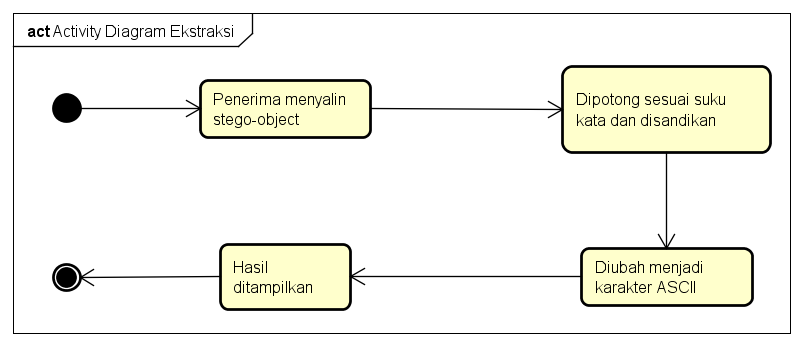
\includegraphics[scale=0.5]{Gambar/activity-ekstraksi}
	\caption{Activity Diagram perangkat lunak steganografi saat proses ekstraksi} 
	\label{fig:4_activity-ekstraksi}
\end{figure}

Dari diagram aktivitas di atas dapat dijelaskan sebagai berikut:

\begin{enumerate}
	\item Pengguna akan memberikan input berupa stego-object dari program yang sama
	\item Sistem lalu akan menyukukan kata-kata yang ada. Setelah itu dilakukan penyandian, angka 0 untuk kata dengan jumlah suku kata genap dan angka 1 untuk jumlah ganjil
	\item Selesai melakukan penyandian, hasilnya akan diubah menjadi karakter ASCII yang sesuai
	\item Kini sudah didapatkan pesan dengan karakter ASCII, hasil akan ditampilkan pada layar
\end{enumerate}